% Created 2017-06-12 Mon 09:39
\documentclass[presentation]{beamer}
\usepackage[utf8]{inputenc}
\usepackage[T1]{fontenc}
\usepackage{fixltx2e}
\usepackage{graphicx}
\usepackage{longtable}
\usepackage{float}
\usepackage{wrapfig}
\usepackage{rotating}
\usepackage[normalem]{ulem}
\usepackage{amsmath}
\usepackage{textcomp}
\usepackage{marvosym}
\usepackage{wasysym}
\usepackage{amssymb}
\usepackage{hyperref}
\tolerance=1000
\usepackage{xeCJK}
\usepackage{minted}
\setCJKmainfont{Source Han Serif SC}
\usetheme[block=fill]{metropolis}
\usecolortheme{metropolis}
\usefonttheme{metropolis}
\useinnertheme{metropolis}
\useoutertheme{metropolis}
\author{金琪琦、刘聪聪}
\date{\today}
\title{JavaScript 代码混淆器}
\hypersetup{
  pdfkeywords={},
  pdfsubject={},
  pdfcreator={Emacs 25.2.1 (Org mode 8.2.10)}}
\begin{document}

\maketitle
\begin{frame}[label=sec-1]{主要内容}
\begin{block}{选题背景}
\end{block}
\begin{block}{设计思路}
\end{block}
\begin{block}{实现简述}
\end{block}
\begin{block}{混淆测试}
\end{block}
\begin{block}{功能演示}
\end{block}
\end{frame}
\begin{frame}[label=sec-2]{选题背景}
\begin{block}{JavaScript}
\begin{itemize}
\item JavaScript 最初被设计用来作为简单的前端脚本
\item 随着前端技术的不断发展,JavaScript 承担了越来越多的功能。它天生安全性不足的缺点得到了充分暴露
\item JavaScript 程序解释执行,整个源代码都暴露在用户面前的特性,决定了代码混淆几乎是现阶段保护 JavaScript 代码唯一有效的手段。
\end{itemize}
\end{block}
\begin{block}{代码混淆}
代码混淆(Obfuscated code)是指将程序代码转换成一种功能上等价,但是难于阅读和理解的形式。
Android 的 apk 就默认使用了代码混淆,使得反编译 APK 变得比较困难。
\end{block}
\end{frame}
\begin{frame}[label=sec-3]{选题背景-意义}
\begin{block}{意义}
\begin{itemize}
\item 前端代码天生的不安全性决定了,应该尽可能将重要的业务代码后移动。
\item 但一方面,总可能会有一些需要在前端处理,又有一定的敏感性业务;
\item 另一方面,前端的一些代码往往是攻击者猜测后端漏洞的入口。
\end{itemize}

因此对于一些重要的前端代码进行适当的混淆,能够增加攻击者破译的难度。保护前端代码的同时维护整个系统的安全。
\end{block}
\end{frame}
\begin{frame}[label=sec-4]{选题背景-现状}
\begin{block}{已有工具}
\begin{itemize}
\item 开源工具:UglifyJS
\item 商业软件:Jscrambler
\end{itemize}
\end{block}
\begin{block}{现状}
目前代码混淆在前端使用得并不多。
\begin{block}{原因}
这并不意味着前端代码不需要保护,或者对前端的代码混淆就没有意义。

而是因为前端的大多数代码并不涉及需要高安全的功能,代码混淆必然导致性能损失,对于轻量级的应用性能比安全更重要。
\end{block}
\end{block}
\end{frame}
\begin{frame}[label=sec-5]{选题背景-应用}
\begin{block}{应用场景}
现在越来越多网站的验证码信息不再仅仅通过一张图片,而是从前端采集用户的操作信息返回给后台判断这一系列操作是否属于人类行为。
面对这样一个前端代码,一旦知道了它的采集策略就很容易伪造信息。因此对这样重要的前端代码进行混淆是很必要的。
\end{block}
\begin{block}{淘宝登录代码}
淘宝登录界面通过 uab.js 程序来采集用户信息,而这个程序就用来加载一个经过混淆的 JavaScript 程序。
\end{block}
\end{frame}
\begin{frame}[label=sec-6]{设计思路}
\begin{block}{合格的代码混淆器}
\begin{enumerate}
\item 人力不可识别
\item 增加自动化还原的难度
\item 增加调试的难度
\end{enumerate}
\end{block}
\begin{block}{实现策略}
\begin{enumerate}
\item 代码混淆
\item 代码防御
\item 代码压缩
\end{enumerate}
\end{block}
\end{frame}
\begin{frame}[label=sec-7]{设计思路-主要模块}
\begin{center}
\begin{figure}[htb]
\centering
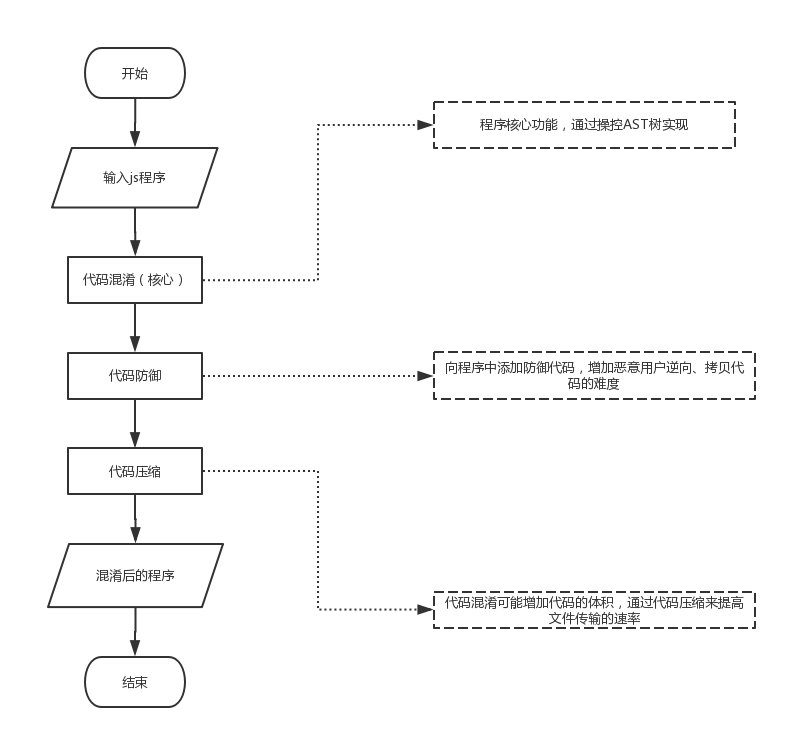
\includegraphics[width=3in]{./presentation03-00.png}
\caption{程序模块}
\end{figure}
\end{center}
\end{frame}
\begin{frame}[label=sec-8]{设计思路-主要原理}
\begin{block}{抽象语法树(AST)}
在源代码的解释和编译过程中,语法分析器创建出抽象语法树,它是源代码的抽象语法结构的树状表现形式,树上的每个节点都表示源代码中的一种结构。一颗抽象语法树展示一个程序的完整语法结构,并不会包含真实语法中出现的每个细节,
\end{block}
\begin{block}{抽象语法树替换}
抽象语法树代表了一个程序的完整语法结构,那么我们可以通过对语法树的调整构造一个功能等效但难以阅读的混淆程序。
\end{block}
\begin{block}{混淆步骤}
\begin{enumerate}
\item 通过某个 JavaScript 引擎解析 javaScript 程序生成 AST;
\item 遍历语法树,并根据适当的混淆规则对语法树进行调整;
\item 通过 JS 引擎将调整后的语法树转换为 JS 源代码,这个代码就是混淆后的代码。
\end{enumerate}
\end{block}
\end{frame}
\begin{frame}[label=sec-9]{设计思路-混淆策略}
\begin{enumerate}
\item 代码混淆
\begin{enumerate}
\item 变量替换
\begin{itemize}
\item 全局变量替换为 window 的属性调用
\item 属性调用替换为取元素操作[]
\item 局部变量名随机化
\end{itemize}
\item 常量混淆
\begin{itemize}
\item 提取所有的字符串,通过字符数组打散
\item 常量编码转换
\end{itemize}
\item 控制流替换
\begin{itemize}
\item 将普通的循环语句展开
\item 将顺序执行的代码放置在精心设计的循环之中
\end{itemize}
\end{enumerate}
\item 代码防御
\begin{enumerate}
\item 禁止控制台调试
\item 域名绑定
\end{enumerate}
\item 代码压缩
\begin{enumerate}
\item 删除注释
\item 删除空白符
\end{enumerate}
\end{enumerate}
\end{frame}
\begin{frame}[label=sec-10]{实现简述-开发环境}
受雅虎开源工具YUI Compressor启发
\begin{block}{开发环境}
\begin{itemize}
\item 平台:Linux
\item 语言:Java
\item IDE:Eclipse
\item 使用了开源 JavaScript 引擎 Rhino
\end{itemize}
\end{block}
\end{frame}
\begin{frame}[fragile,label=sec-11]{实现简述-变量替换}
\begin{block}{源代码}
\begin{minted}{js}
var hello = console.log("hello world");
\end{minted}
\end{block}
\begin{block}{全局变量替换为 window 的属性调用}
\begin{minted}{js}
this.hello = this.console.log("hello world");
\end{minted}
\end{block}
\begin{block}{属性调用替换为取元素操作[]}
\begin{minted}{js}
this["hello"] = this["console"]["log"]("hello world");
\end{minted}
\end{block}
\end{frame}
\begin{frame}[fragile,label=sec-12]{实现简述-字符串转换}
\begin{block}{提取所有的字符串}
\begin{minted}{js}
!function(gin1, gin2, gin3, gin4, gin5) {
  gin1[gin2] = gin1[gin3][gin4](gin5);
}(this, "hello", "console", "log", "hello world");
\end{minted}
\end{block}
\begin{block}{字符数组打散}
\begin{minted}[fontsize=\tiny]{js}

!function(Gin) {
  !function(gin1, gin2, gin3, gin4, gin5) {
  gin1[gin2] = gin1[gin3][gin4](gin5);
}(this, Gin(3, 1, 2, 2, 6), 
Gin(8, 6, 5, 0, 6, 2, 1), 
Gin(2, 6, 7), 
Gin(3, 1, 2, 2, 6, 9, 4, 6, 10, 2, 11));
}(function(Gin) {
  return function() {
  for (var t = arguments, r = "", u = 0, i = t.length; i > u; u++) 
    r += Gin[t[u]];
  return r;
};
}(["s", "e", "l", "h", "w", "n", "o", "g", "c", " ", "r", "d"]));

\end{minted}
\end{block}
\end{frame}
\begin{frame}[fragile,label=sec-13]{实现简述-变量替换}
\begin{block}{局部变量名随机化}
\begin{minted}[fontsize=\tiny]{js}
!function(I) {
  !function(F, L, H, f, _) {
  F[L] = F[H][f](_);
}(this, I(10, 8, 6, 6, 9), I(0, 9, 3, 4, 9, 6, 8), 
I(6, 9, 5), I(10, 8, 6, 6, 9, 7, 1, 9, 11, 6, 2));
}(function(V) {
  return function() {
  for (var B = arguments, c = "", r = 0, $ = B.length; $ > r; r++) 
    c += V[B[r]];
  return c;
};
}(["c", "w", "d", "n", "s", "g", "l", " ", "e", "o", "h", "r"]));

\end{minted}
\end{block}
\end{frame}
\begin{frame}[fragile,label=sec-14]{实现简述-常量编码}
\begin{block}{常量编码转换}
\begin{minted}[fontsize=\tiny]{js}
!function(l) {
  !function(c, B, r, n, D) {
  c[B] = c[r][n](D);
}(this, l(0x8, 0x2, 0x6, 0x6, 0x5), l(0x1, 0x5, 0x0, 0x3, 0x5, 0x6, 0x2),
 l(0x6, 0x5, 0x7), l(0x8, 0x2, 0x6, 0x6, 0x5, 0x9, 0xa, 0x5, 0xb, 0x6, 0x4));
}(function(v) {
  return function() {
  for (var q = arguments, t = "", P = 0x0, $ = q.length; $ > P; P++) 
    t += v[q[P]];
  return t;
};
}(["\u006e", "\u0063", "\u0065", "\u0073", "\u0064", "\u006f", 
"\u006c", "\u0067", "\u0068", "\u0020", "\u0077", "\u0072"]));

\end{minted}
\end{block}
\end{frame}
\begin{frame}[fragile,label=sec-15]{实现简述-代码压缩}
\begin{block}{代码压缩}
\begin{minted}[fontsize=\tiny]{js}
!function(U){!function(z,m,f,g,A){z[m]=z[f][g](A);}(this,U(0x3,0xb,0x7,0x7,0x9),U(0x5,0x9,0xa,0x6
,0x9,0x7,0xb),U(0x7,0x9,0x4),U(0x3,0xb,0x7,0x7,0x9,0x1,0x0,0x9,0x2,0x7,0x8));}(function(k){return
 function(){for(var L=arguments,I="",J=0x0,C=L.length;C>J;J++)I+=k[L[J]];return I;};}(["\u0077","
\u0020","\u0072","\u0068","\u0067","\u0063","\u0073","\u006c","\u0064","\u006f","\u006e","\u0065"
]));
\end{minted}
\end{block}
\end{frame}
\begin{frame}[fragile,label=sec-16]{实现简述-顺序执行变循环}
\begin{block}{顺序执行}
\begin{minted}[fontsize=\tiny]{js}
 var sum = 1 + 2;
 console.log(1);
 console.log(2);
 \end{minted}
\end{block}
\end{frame}
\begin{frame}[fragile,label=sec-17]{实现简述-顺序执行变循环}

\begin{block}{构造循环}
\begin{minted}[fontsize=\tiny]{js}
var _0x2b972d = {
                '\x42\x6c\x67': function _0x160d18(_0xdc9f31, _0x3741dd) {
                    return _0xdc9f31 + _0x3741dd;
                }
            };
var _0x170490 = '\x35\x7c\x34\x7c\x33\x7c\x36'['\x73\x70\x6c\x69\x74']('\x7c'), _0x4f3437 = 0x0;
while (!![]) {
                switch (_0x170490[_0x4f3437++]) {
                case '\x33':
                    console['\x6c\x6f\x67'](0x2);
                    continue;
                case '\x34':
                    console['\x6c\x6f\x67'](0x1);
                    continue;
                case '\x35':
                    var _0x476f51 = _0x2b972d['\x42\x6c\x67'](0x1, 0x2);
                    continue;
                case '\x36':
                    console['\x6c\x6f\x67'](0x5);
                    continue;
                }
                break;
            }
            \end{minted}
\end{block}
\end{frame}
\begin{frame}[fragile,label=sec-18]{实现简述-禁止控制台调试}
在源程序中隐藏插入一段代码,它负责重新定义 console 对象,并抛出异常。当这段代码得以执行 console 就失去了他原来的功能。
\begin{block}{示例代码}
\begin{minted}[fontsize=\tiny]{js}
(function() {  
    try {  
        var $_console$$ = console;  
        Object.defineProperty(window, "console", {  
            get: function() {  
                if ($_console$$._commandLineAPI)  
                    throw "抱歉, 为了用户安全, 本网站已禁用console脚本功能";  
                return $_console$$  
            },  
            set: function($val$_$) {  
                $_console$$ = $val$_$  
            }  
        })  
    } catch ($ignore$$) {  
    }  
})();  
\end{minted}
\end{block}
\end{frame}
\begin{frame}[fragile,label=sec-19]{实现简述-域名绑定}
在源程序中隐藏插入一段代码,它负责监控程序运行时,当前域名是否与既定域名一致,不一致则抛出异常并使程序崩溃退出。
\begin{block}{示例代码}
\begin{minted}[fontsize=\tiny]{js}
(function() {
    var hostname = "www.ustc.com";
    if (location.hostname != hostname) {
        for (key in window) {
        window[key] = undefined;
        }
    throw "js 程序无法在该域名下运行。"
    }
})();
\end{minted}
\end{block}
\end{frame}
\begin{frame}[label=sec-20]{混淆测试}
代码混淆的最基本要求是混淆前后的代码功能上保持一致,这需要测试保证。

\begin{block}{测试环境}
\begin{itemize}
\item 平台:Linux
\item 浏览器:Firefox
\item 回归测试框架:JsUnit
\item 用于测试的Js代码:jQuery
\end{itemize}
\end{block}
\end{frame}
\begin{frame}[label=sec-21]{混淆测试-混淆体积}
\begin{center}
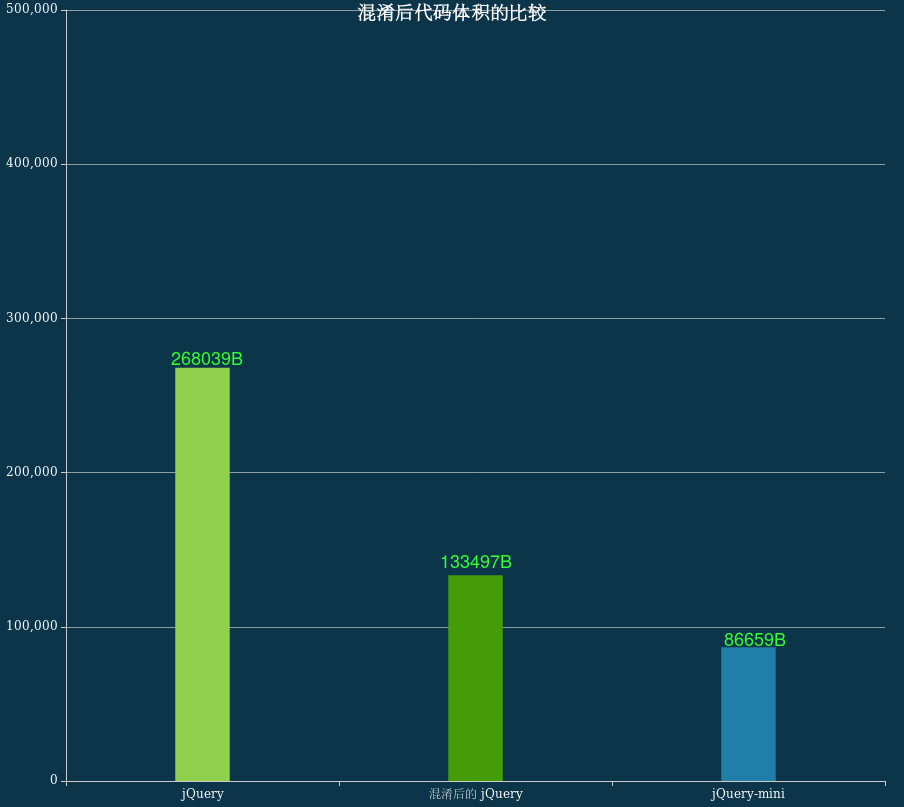
\includegraphics[width=2.8in]{./presentation03-01.png}
\end{center}

对于比较大的js文件,混淆后体积会变小,但和纯粹的压缩代码比起来仍旧比较大。
\end{frame}
\begin{frame}[label=sec-22]{混淆测试}
\begin{center}
\begin{figure}[htb]
\centering
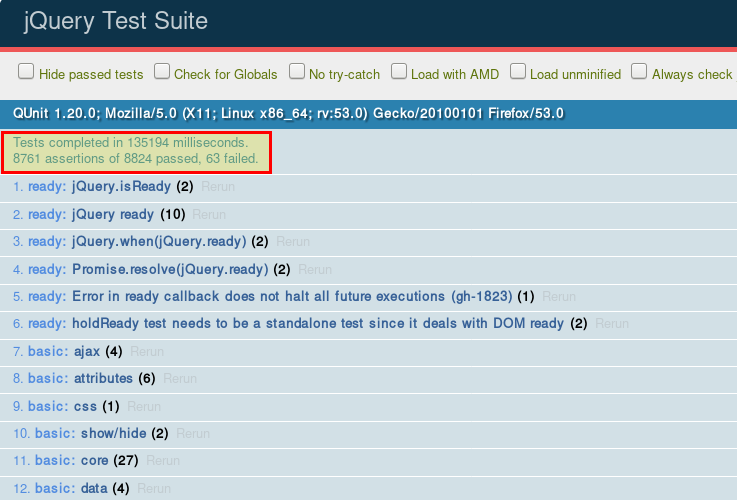
\includegraphics[width=4in]{./presentation03-03.png}
\caption{混淆前}
\end{figure}
\end{center}
\end{frame}

\begin{frame}[label=sec-23]{混淆测试}
\begin{center}
\begin{figure}[htb]
\centering
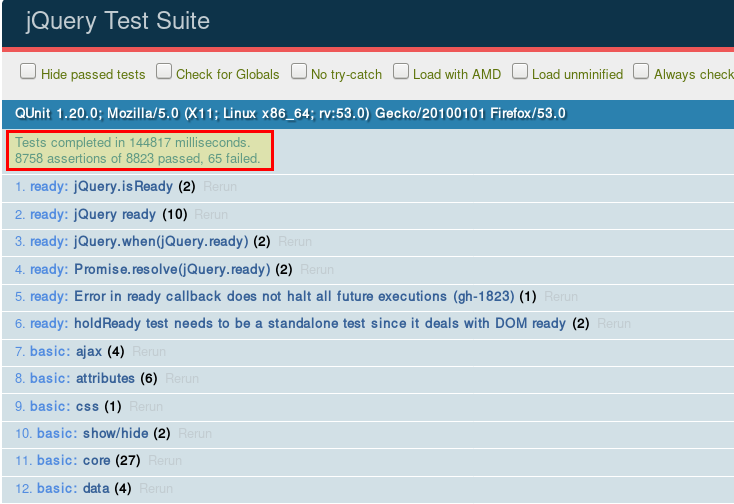
\includegraphics[width=4in]{./presentation03-02.png}
\caption{混淆后}
\end{figure}
\end{center}
\end{frame}

\begin{frame}[label=sec-24]{混淆测试}
\begin{block}{覆盖率}
由于浏览器和系统环境的因素,测试用例覆盖率难以达到100\%。但混淆前后,代码都通过了99\%的测试用例。代码在混淆前后功能的一致性得到了保证。
\end{block}
\begin{block}{运行效率}
混淆后的代码通过测试多用了10000ms,效率降低了10\%。
\end{block}
\begin{block}{总结}
对代码的混淆相当于用时间和空间来交换代码的安全性。因此代码混淆适用于高安全要求而对效率要求不高的场合。
\end{block}
\end{frame}
\begin{frame}[label=sec-25]{功能演示}
该代码混淆器是一个 Java 的命令行程序。通过传递对应的参数和文件名来实现对应的代码混淆功能。
\begin{center}
\begin{figure}[htb]
\centering
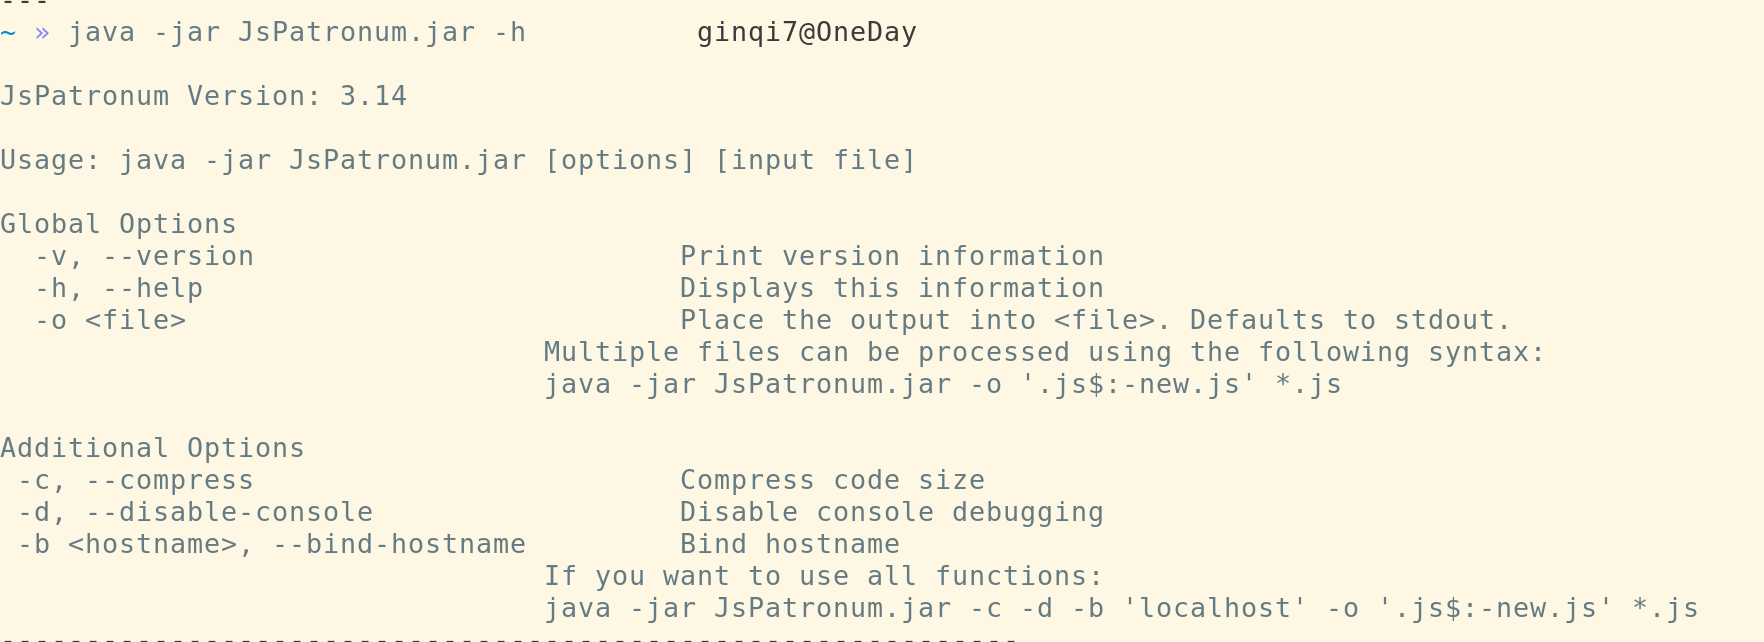
\includegraphics[width=4.5in]{./presentation03-04.png}
\caption{程序帮助}
\end{figure}
\end{center}
\end{frame}
\begin{frame}[label=sec-26]{}
\begin{center}
\Huge{谢谢!}
\end{center}
\end{frame}
% Emacs 25.2.1 (Org mode 8.2.10)
\end{document}